\section{Redis}

In this chapter, we will explore Redis performance. Initially, we will focus on performance under the default configuration. Subsequently, we will explore the scalability of Redis. We will focus on the impact of multiple instances running simultaneously under various load configurations. Unless otherwise stated, all benchmarks will be performed such that they meet the desired Quality of Service (QoS) defined as having 99th percentile latency under 1 millisecond.

\subsection{Out of the Box Performance}
Firstly, let us focus on the performance characteristics Redis achieves without any special configuration enabled. Once deployed to a server, a Redis server can be started with the following:
\begin{lstlisting}
redis redis.conf --port 11120
\end{lstlisting}

The \texttt{redis.conf} refers to a configuration file which is part of the official distribution \cite{RedisConfiguration}. Any arguments prefixed with \texttt{--} will overwrite the settings inside \texttt{redis.conf}. In our case, we are setting the port to listen on 11120. Otherwise, all configuration remains unmodified.

The clients are setup in order to produce an increasing load on Redis. In order to do this, we increase the number of connections each client will utilize to send requests to the Redis server. The number of connections is increased at a constant rate of 1. Note that we utilize the \texttt{-P} argument to specify we are interested in benchmarking Redis.

\begin{lstlisting}
memtier -s nsl200 -p 11120 -c <connection_count> -t 2 -P redis
--random-data
--key-minimum=100
--key-maximum=10000
\end{lstlisting}

\begin{figure}[h]
    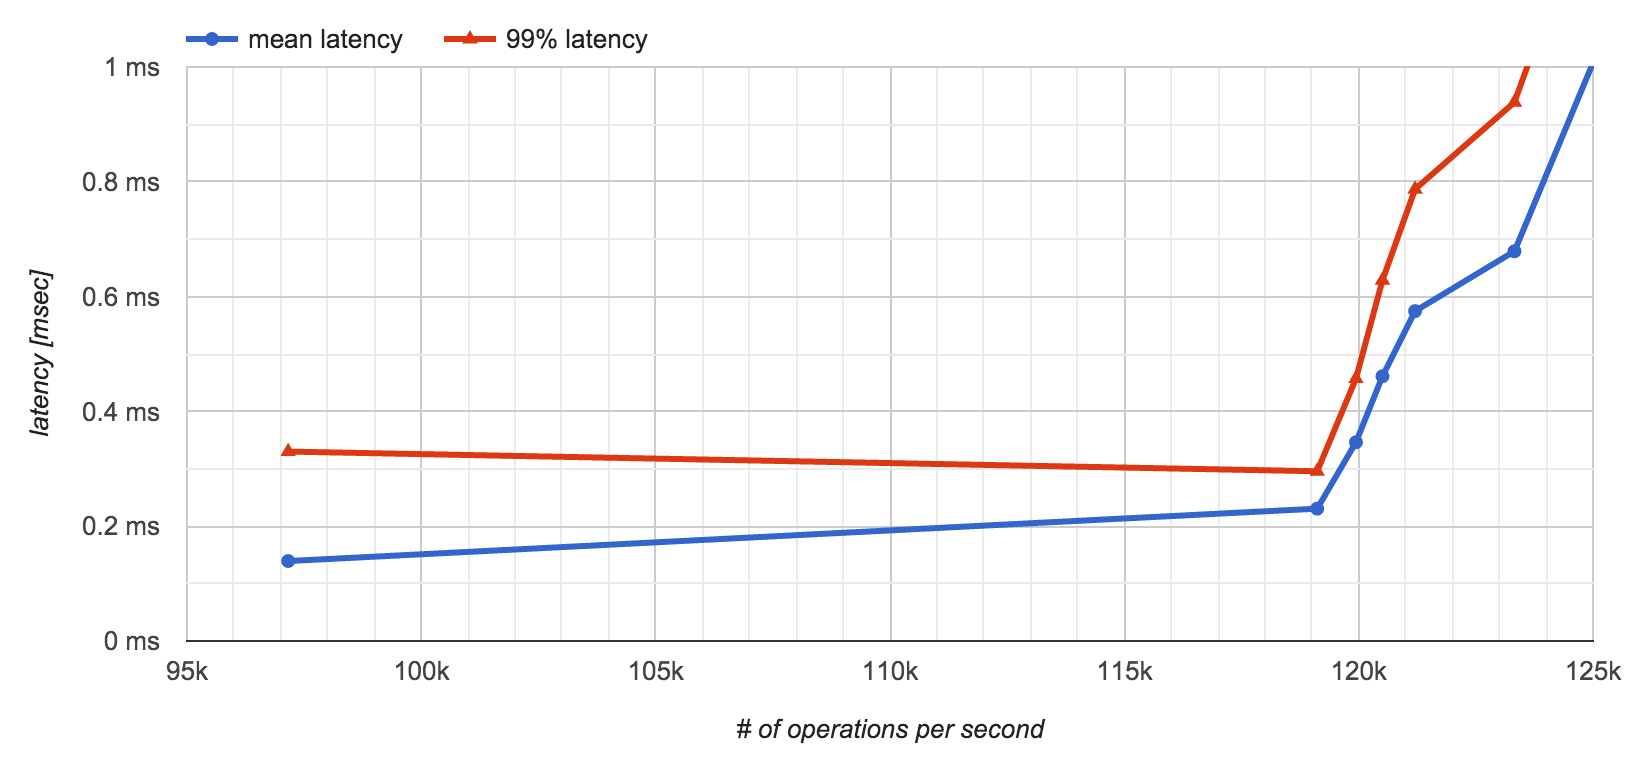
\includegraphics[width=\textwidth]{./res/6_default_latency_ops.png}
    \caption{Redis: Throughput vs Mean and 99th percentile latency}
    \label{fig:redis-default-latency-ops}
\end{figure}

Figure \ref{fig:redis-default-latency-ops} shows the relationship between mean and 99th percentile latency on the vertical axis and the number of operations per second on the horizontal axis. The graph has been trimmed to show only data which satisfies the QoS requirements. We can observe that the number of operations Redis processes increases steadily until it reaches 119k requests per second at which point a further increase in throughput comes at a disproportionately grater cost in latency. The peak throughput observed under the QoS requirements is 125,000 requests per second.